\documentclass{standalone}
\usepackage{tikz}
\usepackage{ctex,siunitx}
\setCJKmainfont{Noto Serif CJK SC}
\usepackage{tkz-euclide}
\usepackage{amsmath}
\usepackage{wasysym}
\usetikzlibrary{patterns, calc}
\usetikzlibrary {decorations.pathmorphing, decorations.pathreplacing, decorations.shapes}
\begin{document}
\small
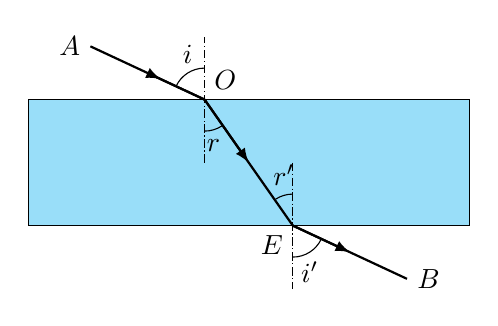
\begin{tikzpicture}[>=latex,scale=0.8]
  \draw [fill=cyan!40] (-3.5,-2) rectangle (3.5,0);
  \draw [thick](-0.7,0)--(0.7,-2);	
  \node at (-.7,0)[above right]{$O$};
  \node at (.7,-2)[below left]{$E$};
  \draw[->,thick](-0.7,0)--(0,-1)	;
  \draw[thick] (-0.7,0)--+(155:2)node [left]{$A$};
  \draw[thick] (0.7,-2)--+(-25:2)node [right]{$B$};
  \draw[thick, -<] (-0.7,0)--+(155:1);
  \draw[thick, ->] (0.7,-2)--+(-25:1);
  \draw[densely dashdotted] (-0.7,-1)--(-0.7,1);
  \draw[densely dashdotted] (0.7,-1)--(0.7,-3);
  \draw (-0.7,0.5) arc (90:155:.5)node[midway,above]{$i$};
  \draw (0.7,-2.5) arc (-90:-25:.5)node[midway,below]{$i'$};
  \draw (-0.7,-0.5) arc (-90:-57:.5)node[midway,below]{$r$};
  \draw (0.7,-1.5) arc (90:123:.5)node[midway,above]{$r'$};
\end{tikzpicture}
\end{document}